% !TeX root = ../main.tex

\section{Automazione del Processo di Sviluppo}

\begin{frame}{Processo di sviluppo}

    \begin{figure}[H]
        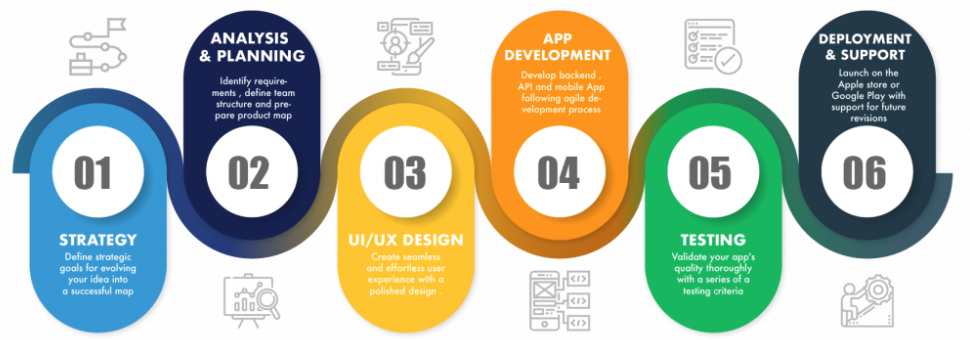
\includegraphics[width=1\textwidth]{img/sdlc2.png}
    \end{figure}

\end{frame}

\begin{frame}{Pratiche DevOps}
    \begin{columns}[onlytextwidth,t]
        \begin{column}{0.33\textwidth}
    
            \textbf{Continuous Integration}
            \vspace{2mm}
            \begin{itemize}
                \item \textbf{Principio}: Integrazione frequente di piccole modifiche, testate automaticamente
                \vspace{2mm}
                \item \textbf{Stages}:
                \begin{itemize}
                    \item Build
                    \item Test
                    \item Package
                \end{itemize}
            \end{itemize}
            
        \end{column}
        \begin{column}{0.33\textwidth}

            \textbf{Continuous Delivery}:
            \vspace{2mm}
            \begin{itemize}
                \item \textbf{Principio}: Rilascio frequente di piccole modifiche, eseguito in modo automatico \newline
                \vspace{2mm}
                \item \textbf{Stages}:
                \begin{itemize}
                    \item Release alpha
                    \item Release beta
                    \item Release prod
                \end{itemize}
            \end{itemize}
        
        \end{column}
        \begin{column}{0.33\textwidth}

            \textbf{Continuous Inspection}
            \vspace{2mm}
            \begin{itemize}
                \item \textbf{Principio}: Analisi automatica del codice per garantire un certo livello di qualità e di sicurezza
                \vspace{2mm}
                \item \textbf{Stages}:
                \begin{itemize}
                    \item Analisi statica
                    \item Analisi dipendenze
                \end{itemize}
            \end{itemize}
        
        \end{column}
    \end{columns}

    \vspace{6mm}

    \begin{figure}[H]
        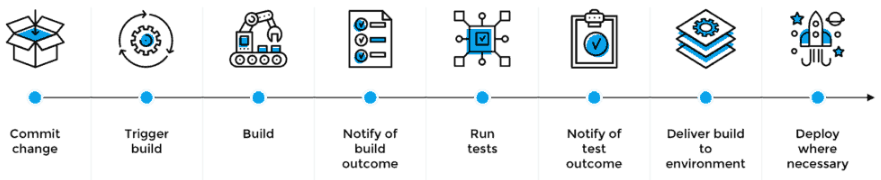
\includegraphics[width=0.9\textwidth]{img/cicd.png}
    \end{figure}

\end{frame}